%% This skeleton file requires IEEEtran.cls version 1.6 or later.
%%
\documentclass[conference,letterpaper]{IEEEtran}
% If the IEEEtran.cls has not been installed into the LaTeX system files,
% manually specify the path to it:
%\documentclass[conference]{../sty/IEEEtran}
\IEEEoverridecommandlockouts
\overrideIEEEmargins

% some very useful LaTeX packages include:

\usepackage{cite}      % Written by Donald Arseneau
                        % V1.6 and later of IEEEtran pre-defines the format
                        % of the cite.sty package \cite{} output to follow
                        % that of IEEE. Loading the cite package will
                        % result in citation numbers being automatically
                        % sorted and properly "ranged". i.e.,
                        % [1], [9], [2], [7], [5], [6]
                        % (without using cite.sty)
                        % will become:
                        % [1], [2], [5]--[7], [9] (using cite.sty)
                        % cite.sty's \cite will automatically add leading
                        % space, if needed. Use cite.sty's noadjust option
                        % (cite.sty V3.8 and later) if you want to turn this
                        % off. cite.sty is already installed on most LaTeX
                        % systems. The latest version can be obtained at:
                        % http://www.ctan.org/tex-archive/macros/latex/contrib
%/supported/cite/

\usepackage[dvips]{graphicx}  % Written by David Carlisle and Sebastian Rahtz
                        % Required if you want graphics, photos, etc.
                        % graphicx.sty is already installed on most LaTeX
                        % systems. The latest version and documentation can
                        % be obtained at:
                        % http://www.ctan.org/tex-archive/macros/latex/required/graphics/
                        % Another good source of documentation is "Using
                        % Imported Graphics in LaTeX2e" by Keith Reckdahl
                        % which can be found as esplatex.ps and epslatex.pdf
                        % at: http://www.ctan.org/tex-archive/info/

%\usepackage{amsmath}   % From the American Mathematical Society
                        % A popular package that provides many helpful commands
                        % for dealing with mathematics. Note that the AMSmath
                        % package sets \interdisplaylinepenalty to 10000 thus
                        % preventing page breaks from occurring within multiline
                        % equations. Use:
%\usepackage{amssymb}
\usepackage{subfigure}
\usepackage{multirow}
\usepackage[left=0.71in,top=0.94in,right=0.71in,bottom=1.18in]{geometry}
\setlength{\columnsep}{0.24in}
% correct bad hyphenation here
%\hyphenation{op-tical net-works semi-conduc-tor IEEEtran}

%New theorems
\newtheorem{fact}{Proposition}
\newtheorem{definition}{Definition}
%New commands
\newcommand{\q}{\mathbf q}
\newcommand{\dq}{\dot {\mathbf q}}
\newcommand{\deltauhand}{\Delta \mathbf {u}_{hand}}
\newcommand{\deltaqarm}{\Delta \mathbf {q}_{arm}}
\newcommand{\qarm}{\mathbf q_{arm}}
\newcommand{\jacobian}{\mathbf J}
\newcommand{\uhand}{\mathbf{u}_{hand}}
\newcommand{\utarget}{\mathbf{u}_{target}}
\newcommand{\xhand}{\mathbf{x}_{hand}}
\newcommand{\qhead}{\mathbf{q}_{head}}
\newcommand{\xtarget}{\mathbf{x}_{target}}

\begin{document}
% paper title
\title{\huge A novel approach to manipulation (tentative title)}

% author names and affiliations
\author{\authorblockN{Eduardo Torres-Jara}
\authorblockA{
\textit{MIT}\\
\textit{Mass Ave}\\
\textit{email}\\}
\and
\authorblockN{Lorenzo Natale}
\authorblockA{
\textit{Italian Institute of Technology}\\
\textit{Via Morego 30, Genova, ITALY}\\
\textit{lorenzo.natale@iit.it}\\}
}

% make the title area
\maketitle
\begin{abstract}
Many of the useful tasks, that humans do, involve the use of their
hands to manipulate objects. We control our hands very dexterously
in a variety of environments daily. However, state of the art
robots are very limited at the moment of manipulating the same
objects. For instance, a robot can precisely position a part, but
it is not capable of picking up objects from a box or even
grabbing an object from a table. Part of the reason for that
limited performance of robot manipulation is the current approach
that relies in a prebuilt model and a precise arm. Here, we
present an alternative and effective approach to manipulation that
we call sensitive manipulation. This approach uses massive sensing
and a soft hand to actually come in contact with the objects to
manipulate specifically and the environment in general. As a
result, the robot Obrero, is capable of reaching for unknown
objects, reorient its hand to grab the object, apply enough force
to avoid slippage when moving the object and place an object in a
surface. These operations are done using mainly tactile feedback
and they are adaptive to object shapes and surfaces. Besides, it
is greatly reduces the computation needed in comparison to a
traditional approach. Thus, Sensitive Manipulation, makes possible
for robots to be more dexterous and adaptive when manipulating
objects[fisrt attempt]

\end{abstract}

% key words
\begin{keywords}
Keywords.
\end{keywords}
%
\section{Introduction}
Put here the introduction.
%




%% Later on in development the integration between visual and tactile
%% modalities during reaching tasks has been found. Tactile
%% information is, for example, used to confirm visual stimulus as
%% described in \cite{bower70Coordination}. In this experiment an
%% image of an object was projected used polarized lenses so that
%% children wearing ``stereo'' glasses perceived a 3D object.
%% Children of different ages were tested in two conditions: when the
%% object was actually present and when it was not. Older children (5
%% to 6 months-old) showed surprise when the did not feel the contact
%% when expected, whereas the younger ones closed their hand to grasp
%% the object \textbf{[X and  did not show any surprise. * This is
%% not true. Both showed surprise. Also, I am not sure if its later
%% because the experiment was done with children from 6 days to 6
%% months. And we do not know if they were tested in the both
%% conditions. X]}
%

\section{Grasping, lifting and placing an unknown object}
\label{sec:controlling}
%
\subsection{Experiment setup} In this implementation we have a
table(flat and horizontal) in front of the robot OBRERO. The table
is reachable by the robot's hand. Objects are presented by a
person on this table. The robot does not have a model of the
objects presented.
%
The robot initially detect the presence of the table and determine
its height. (low friction)
%
The robot's attention is captured by moving an object in the
table. The robot's response is to move its hand toward the object,
grab it, lift it and placed in an surface.
%
The object can be placed anywhere within reach of the robot's
hand.
%


%\section{Robot and Tactile feedback}

\subsection{Grasping an object}
\label{sec:impbehavior}

\begin{figure*}[htbp]
\centerline{
\includegraphics[width=2.8in, angle=270 ]{./figures/GrabSeq.eps}
} \caption[An example of the Grasping Behavior]{Grasping behavior:
an example. Sequence of the robot grasping a porcelain cup. Frame
1: the cup is presented to the robot. Frame 2: the robot reaches
for the cup. Frames 3 to 6: the robot explores the space and uses
tactile feedback to find the object and adjust the position of the
hand. Frames 7 and 8: the robot grasps and lifts the cup.}
\label{fig:sequence}
\end{figure*}

We assume that the robot's arm starts at a position above the
table. The hand has its thumb up and the index and middle fingers
extended. When a person waves an object(motion
detection\cite{kemp-thesis}) in front of the robot, the robot
moves its hand towards the object using the 2D information of the
camera and the kinematics information from the head and the arm.
The third dimension is given by the height of the table that the
arm originally detected.

After the reaching motion and if not contact has been detected, an
exploration around this position is performed. The hand is moved
to the side and to the front parallel to the table. These
directions are computed using the kinematics of the arm.

If contact with the hand is detected, the exploration is stopped
and the thumb is rotated to oppose the index finger. Then, the
hand is repositioned depending on where the contact occurred.(*)
If only the index finger is in contact with the object, the hand
is moved down until contact with the table.
%
If there is not contact with the palm, the arm will be moved in
the direction of the forearm until contact occurs.
%
Once in contact with the palm, the fingers will be closed ...
%
If the operation fails a the arm will be returned to the initial
position.

\subsection{Lifting an object and slippage detection}
%\subsection{Slippage}
In order to apply enough force to lift an object, we detect if it
slips.

%Although controlling slippage can be useful in several
%manipulation tasks, we focus on avoiding slippage when lifting.

Sensing slippage is not an straight-forward task since the
phenomena is not quite understood. If we observe humans, our skin
has innervations that respond to fast motions on the surface.
These innervations are the Meissner's corpuscles. They are
specialized on detecting vibrations. Those vibrations are, in
principle, related to the catch and release effect caused by an
object sliding on the surface of the skin. This has inspired other
researchers to build tactile sensors with the capability of
detecting vibrations using accelerometers\cite{howe89sensing}.

In our case we do not rely on this principle. Instead, we measure
the change of the force applied on the direction of the lifting.

We illustrate this principle on the following experiment. We use
the the cylindrical bottle ($mass=0.179 Kg$, $diameter=92 mm$,
$height=216 mm$) shown in figure~\ref{fig:slipseq}. The robot
approaches the bottle by the side, touches it and subsequently
rotates the thumb to grab the object. Since it is the first time
it works with the bottle, it closes its thumb and index finger
gently until contact with the object is detected. At this point,
it closes the fingers more to deflect the sensors. This is
necessary in order to obtain reliable readings from forces applied
in directions parallel to the base of the sensors. In
figure~\ref{fig:tactileref} we can observe the direction of the
forces on the tactile sensors. In this experiment, we use only the
tactile sensors on the distal phalanges of the fingers. The force
normal to the tactile sensor surface is in the X direction, and
the ones parallel are in the plane Y-Z.

When the fingers are closed on the object, the forces in X
increase. The forces in Z (on the direction of gravity) and the
forces in Y also change due to the deformation of the sensors.
This deformation depends, at this point, on the angle of incident
between the tactile sensor and the surface of the object and not
on the weight.

When the robot starts moving its hand upwards, that is indicated
by the increment of elbow angle figure~\ref{fig:slip}, the force
in Z increases in magnitude because the weight of the object pulls
the sensors down. Assuming that the motion is linearly upwards and
that the object does not rotate, the force should remain somewhat
stable. The exception is at the beginning of the lifting where the
dynamics of the motion are noticeable. The event just described is
illustrated on the right side of figure~\ref{fig:slip}.

On the left side of figure~\ref{fig:slip}, we see that the
behavior is different. The total force goes back to zero while the
fingers are still closed. This is because the object slipped from
the hand. A sequence of images of the slippage is shown in
figure~\ref{fig:slipseq}. It is important to notice in this figure
that the bottle moves downwards but also towards the front. That
is, the bottle rotates on the finger tips of the hand.

If we now return to figure~\ref{fig:slip}, we can see the dynamics
of the sensors/object interaction. After the point B, in the
figure, the total force becomes negative because the friction with
the object pulls the sensors down. This event is indicated by an
increment on the elbow angle. While the total force is negative,
there is a slight positive slope on the force that indicates some
slippage. But more importantly, the angle between forces Z and Y
in the thumb changes smoothly showing the rotational slippage.
Subsequently, the object stops pulling down the tactile sensors
when it touches the table. At point C in figure~\ref{fig:slip},
the fingers are opened.


In order to detect slippage, we observe the total tactile force
while the fingers are closed and the arm moves upwards. If we
detect a positive slope, we conclude that there is slippage. We
can observe this in figure~\ref{fig:slip}. From point B to C there
is a large positive slope. The slope is presented on the top plot
for reference. From points E to F, there is a slight slip that
stops and the grasp stabilizes.

The response time of this slip detector is not as fast as it would
be required to adjust the force instantly. Instead, a new attempt
to lift the object is done if slippage has been detected.

[The current limitation of these sensors is that computation is
done off-board. However, the hardware on the sensors have the
capability of doing this calculation faster.]


\begin{figure}[htbp]
\centerline{
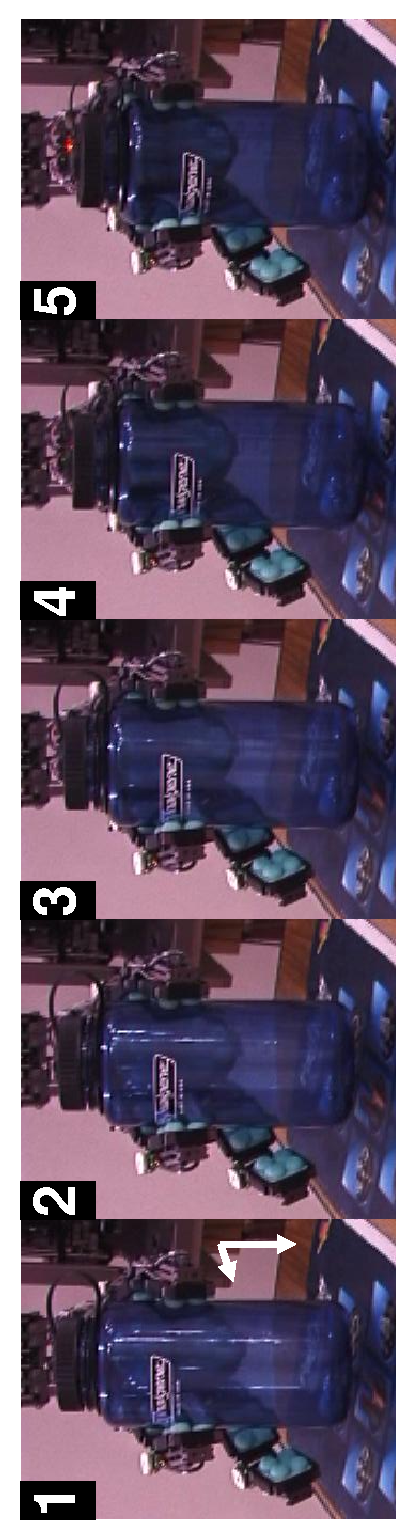
\includegraphics[height=\columnwidth, angle=270 ]{./figures/Slippage.eps}
} \caption[Bottle slipping]{From 1 to 5 we observe the bottle
slipping. The bottle moves downwards and towards the front. The
motion towards the front is not linear but circular.}
\label{fig:slipseq}
\end{figure}


It is important to remember that the data comes from a controlled
experiment where the lifting is done only with the thumb and the
index finger. Neither the palm nor the middle finger are used. In
general, this robot is designed to do whole body grasping as
opposed to precision grasping. In some cases, an object will come
in contact with the fingers on spots where the fingers are not
fully covered with the skin. In that case the slippage detection
is not possible.

\begin{figure*}[htbp]
\centerline{
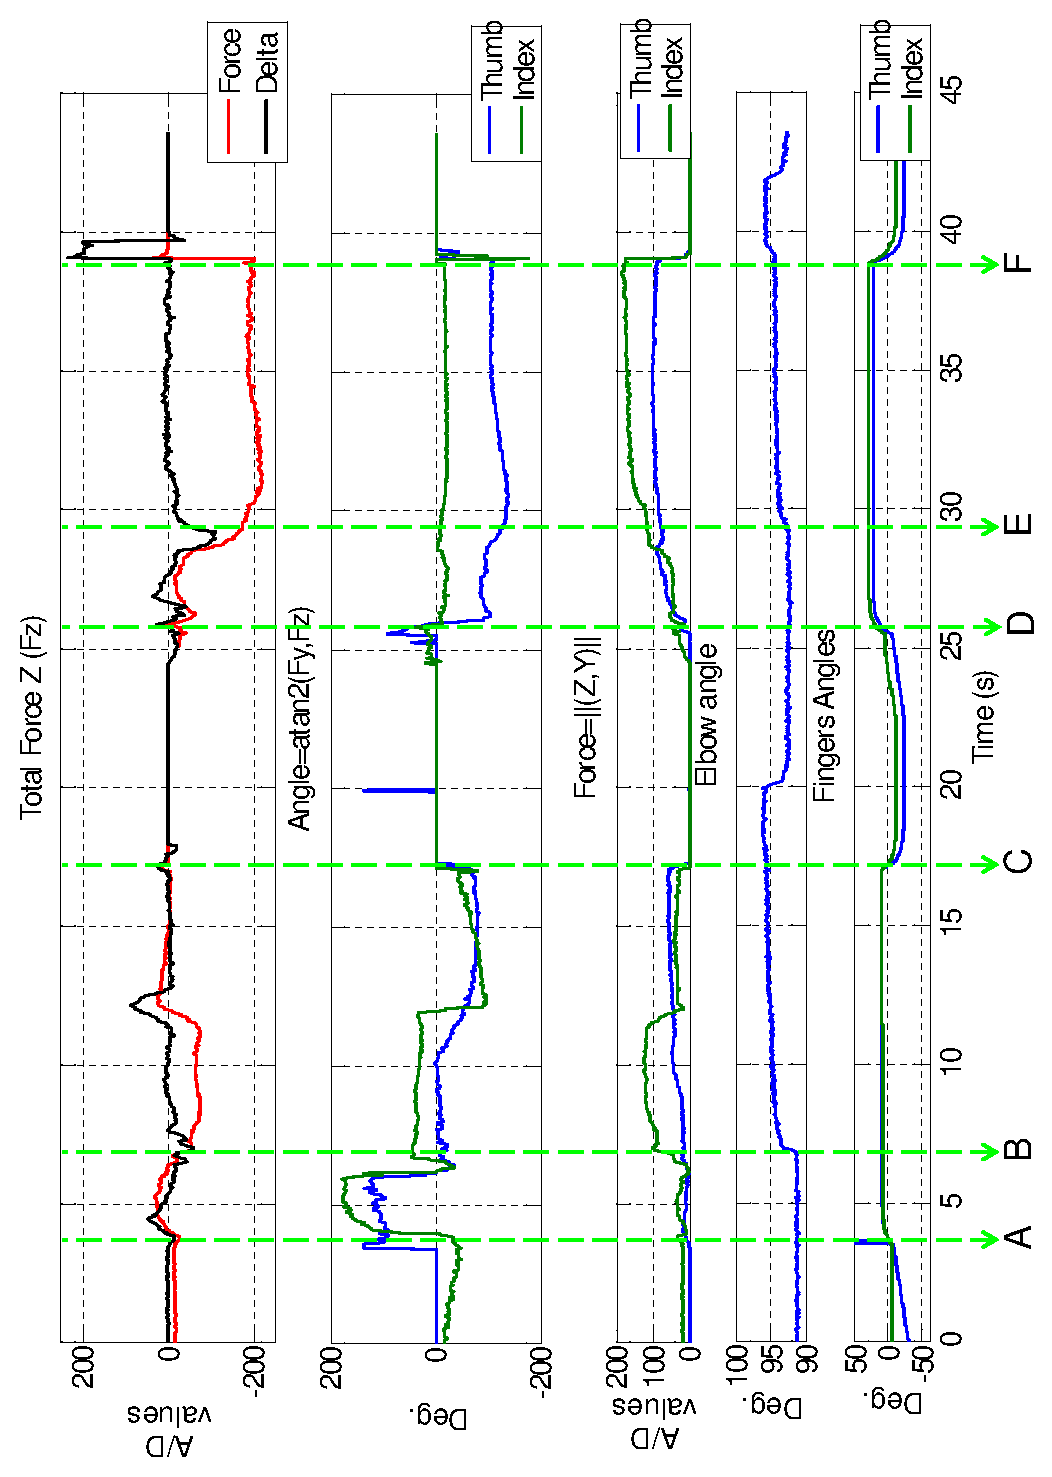
\includegraphics[height=\textwidth, angle=270 ]{./figures/ThesisSlipX.eps}
} \caption[Tactile forces when lifting an object]{Tactile forces
in two different lifting events. For details see
section~\ref{sec:slippage} } \label{fig:slip}
\end{figure*}

\subsection{Placing an object on a surface: applying forces to a held object}

Once the robot has an object in its hand, in order to interact
with the environment it is important to detect changes of forces
applied to the object. For instance, if the robot is holding an
object and wants to place it on a flat surface, like a table, it
is important to detect when they come in contact so an action can
be taken. Other examples where detecting external contact with a
held object include: using a hand tool, moving a cup towards our
mouth, etc.

OBRERO's tactile sensors are capable of measuring changes on the
forces applied to the object. In order to illustrate the principle
we present the following example. The robot grabs the bottle used
in section~\ref{sec:slippage}. Subsequently, it lifts the bottle
and then moves it back to the surface. The forces applied to the
object are monitored using the tactile sensors. When a large
change on the forces is detected in direction opposite to the
motion, the robot assumes that the object came in contact with a
surface and releases its grip. The robot is capable of detecting
this change at any time. For example, if we place our hand under
the bottle before the robot touches the surface, the robot will
able to detect this change on the tactile forces. This example is
presented in figure~\ref{fig:landing}.


It is arguable that this detection can also be done by force
sensors on the joints of the robot. However, this is generally
less sensitive because the effect of the change on forces needs to
be reflected on the joint. More importantly, a detailed model of
the forces acting on the joints needs to be implemented in order
to filter out the changes produced by other factors. Tactile
sensors are closer to the hand/object interaction making them more
sensitive and less complex at the moment of extracting the
information.

Figure~\ref{fig:twotaps} shows the response of the tactile sensors
to external forces on the object held. In this case, the robot is
holding an object and a person pushes the object from the bottom.
In order to see the response, we program the robot so that it does
not release the object. The plot on the top of
figure~\ref{fig:twotaps} shows the changes on the forces in the
direction of gravity.  We do not work with the absolute force but
with the differences because we are interested in the changes on
the force. The values showed have been filtered using a moving
average filter of size 8 and the sampling period is 100ms. The
bottom plot on figure~\ref{fig:twotaps} is the integration of the
data on the top plot, and it gives an idea of the time evolution
of the force applied. We can clearly observe that the force
increased because the object was pushed twice and the forces
applied had different intensity.

In order to detect the event of pushing or contacting the table
setting a threshold is enough, as it is illustrated on the top
plot of figure~\ref{fig:twotaps}.


\begin{figure}[htbp]
\centerline{
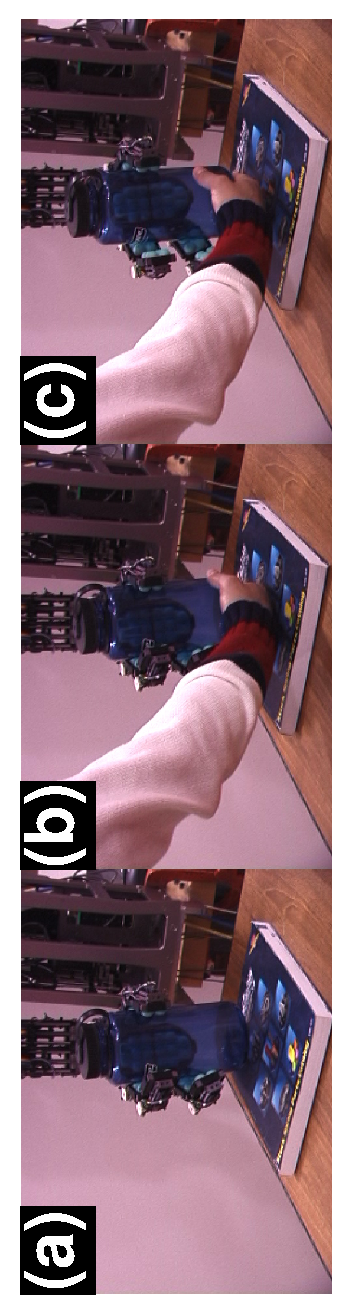
\includegraphics[height=\columnwidth, angle=270 ]{./figures/SeqHandDelivery.eps}
} \caption[Detection of forces applied to an object held by the
robot]{This sequence shows the robot detecting forces applied over
an object when holding it. This is useful to place objects over
surfaces. In (a) the robot is holding a bottle, in (b) a person is
touching the bottle from below and the robot detects this force.
As a consequence, the robot releases the object as shown in (c)}
\label{fig:landing}
\end{figure}


\begin{figure}[htbp]
\centerline{
\includegraphics[height=\columnwidth, angle=270 ]{./figures/2TapsX.eps}
} \caption[Pushing the bottle upwards twice]{Pushing the bottle
upwards twice. Top: Temporal difference of the total force in
direction on the gravity when the hand is holding an object. See
figure~\ref{fig:tactileref} for reference. Bottom: Integration of
the data on the top plot. It shows the changes on force when the
object was pushed.} \label{fig:twotaps}
\end{figure}









%
%\begin{figure}[htbp]
%  \centering
%  \subfigure{
%    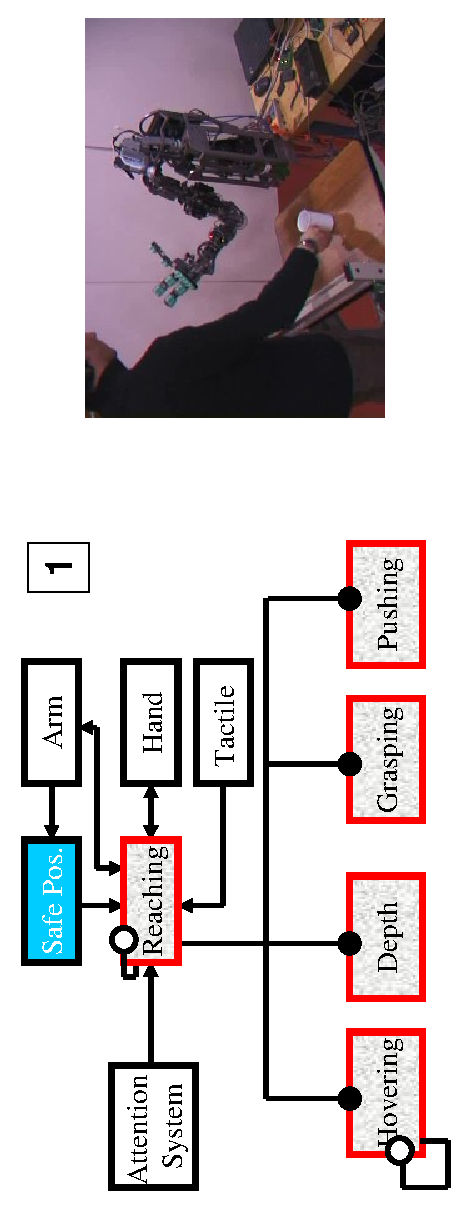
\includegraphics[height=\columnwidth, angle=270]{./figures/bstep1.eps}}
%    \hfill
%    \subfigure{
%    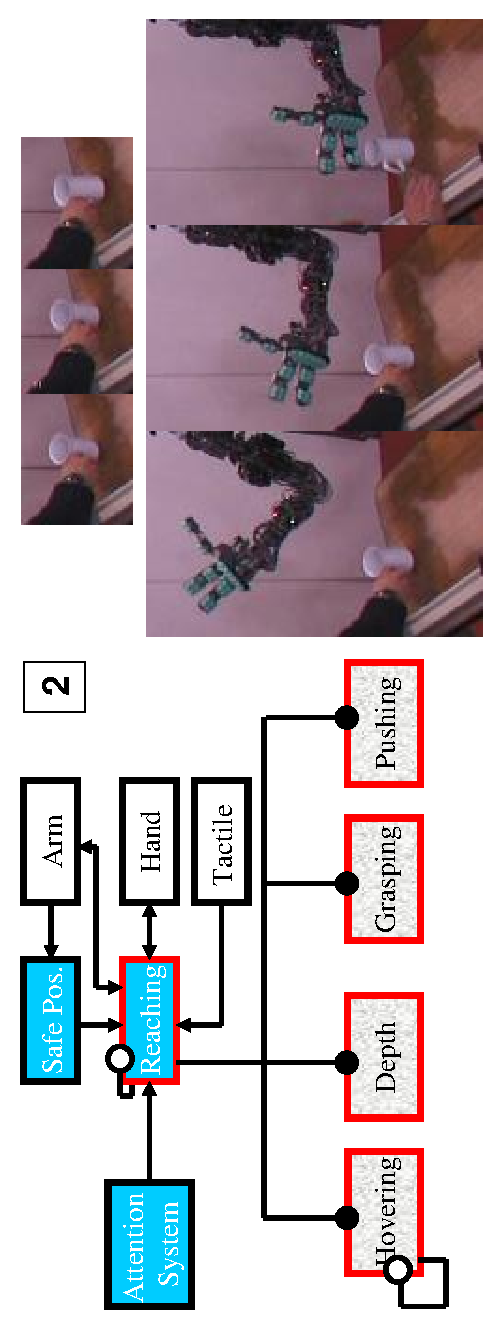
\includegraphics[height=\columnwidth, angle=270]{./figures/bstep2.eps}}
%        \hfill
%        \subfigure{
%    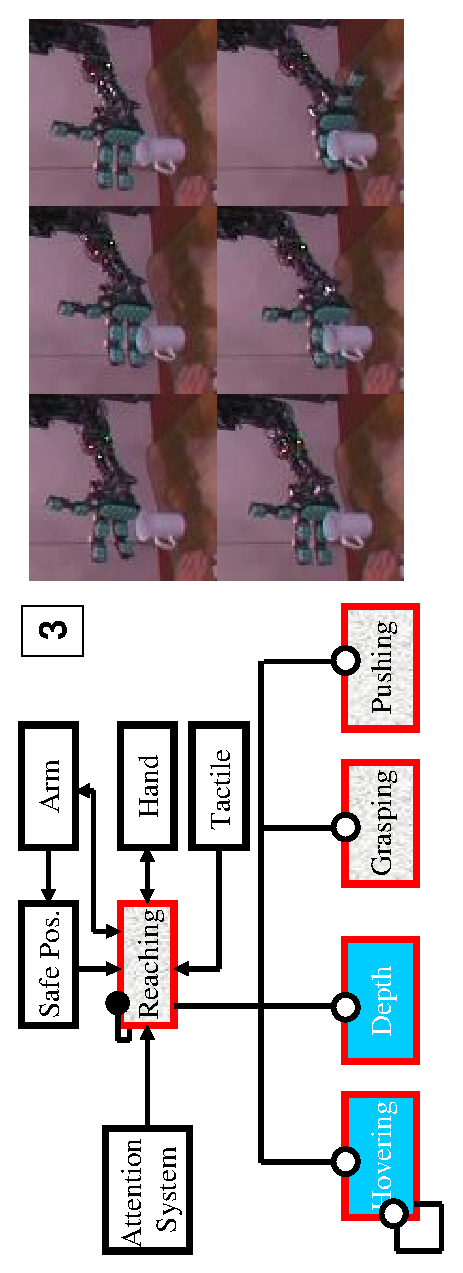
\includegraphics[height=\columnwidth, angle=270]{./figures/bstep3.eps}}
%        \hfill
%        \subfigure{
%    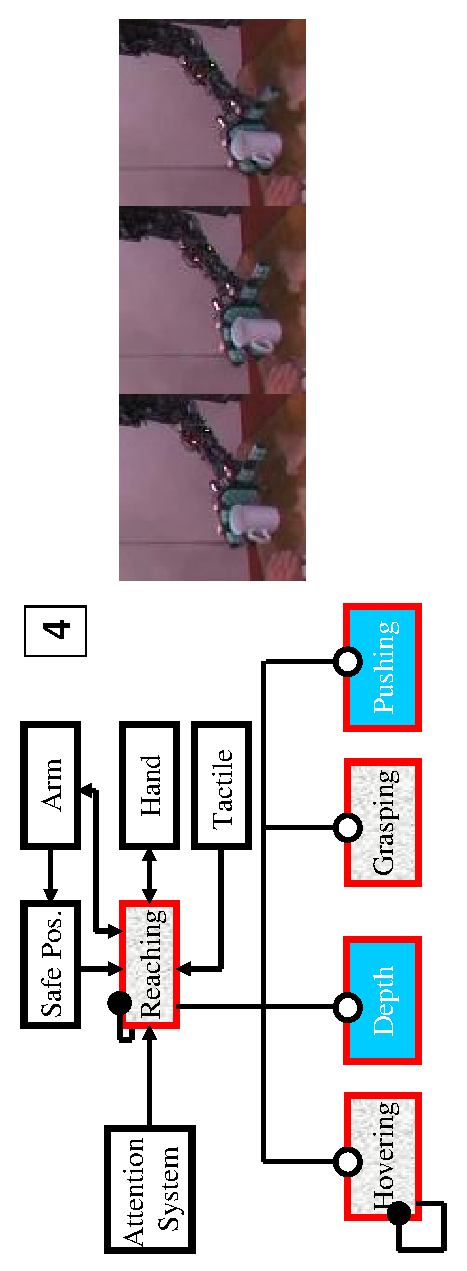
\includegraphics[height=\columnwidth, angle=270]{./figures/bstep4.eps}}
%
%  %
%  \caption[Behaviors and robot's actions]{From top to bottom, we
%  observe a sequence of the behaviors' activity  and the generated
%  robot's actions. The explanation of the behaviors is presented in
%  figure~\ref{fig:expbehaviors}. 1. The arm is in the safe
%  position. 2. The cup is being shaken and the arm reaches toward
%  the cup. 3. The arm moves side to side and downwards. 4. The arm
%  moves toward the cup.
%  } \label{fig:bsteps}
%\end{figure}

\section{Evaluations}
\label{sec:results}

\begin{table*}[htb]
  \caption{Objects.} \label{tab:objects} \centering
  \begin{tabular}{|c|l|c|c|c|l|}
    \hline
    &Description& Weight(Kg)&No.Trials&No.Failures&Contains \\
    %&Object& W(Kg)&Trials&Fail&Contains \\
    \hline
    1&Plastic bottle        & 0.265 & 22& 0 & Vitamins\\
    2&Porcelain cup & 0.255 & 24& 1 & Nothing\\
    3&Plastic cup (Starbucks)      & 0.220 & 24& 4 & Bolts \\
    4&Rectangular box (Nesquick)        & 0.240 & 24& 2 & Nesquick powder\\

    \hline
  \end{tabular}
\end{table*}

\begin{figure*}[tbp]
\centerline{
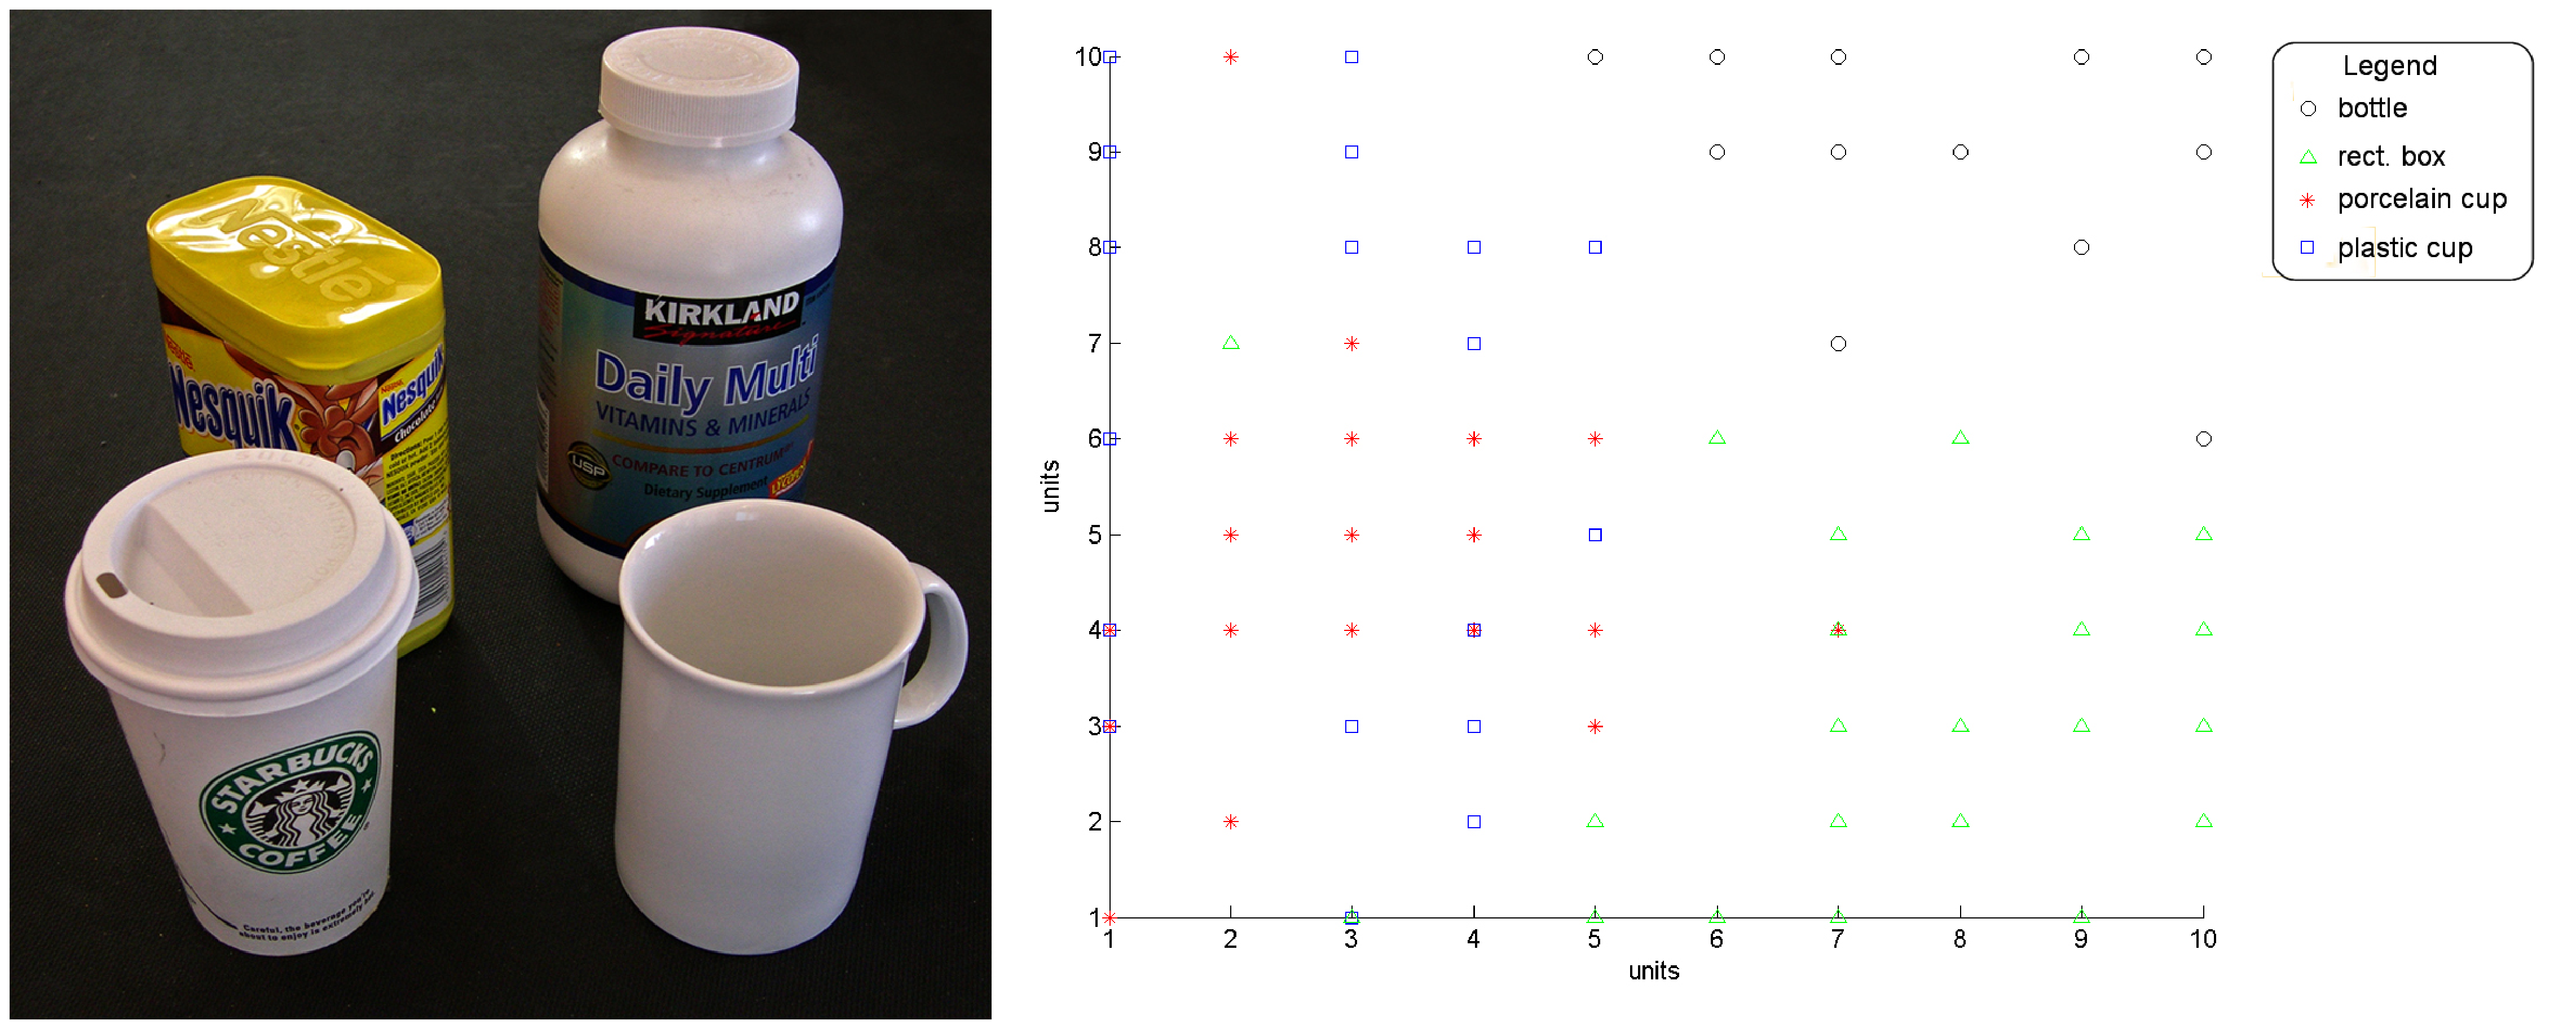
\includegraphics[width=6.0in]{./figures/objects-clusters2.eps}
}\caption[Objects grabbed and clustering]{Left: the set of objects
used in the experiments: a plastic bottle, a porcelain cup, a
plastic cup and a rectangular plastic box. Some objects were
partially filled to increase the weight (all objects weighed about
220-250g). Right: result of the clustering. Black circles, green
triangles, red stars and blue squares represent respectively the
bottle, the rectangular box and the porcelain and the plastic
cups. The two cups are not clearly separated because they have
similar shape in the area where they were grasped.}
\label{fig:Objects}
\end{figure*}

%% \begin{figure}[tbp]
%% \centerline{
%% 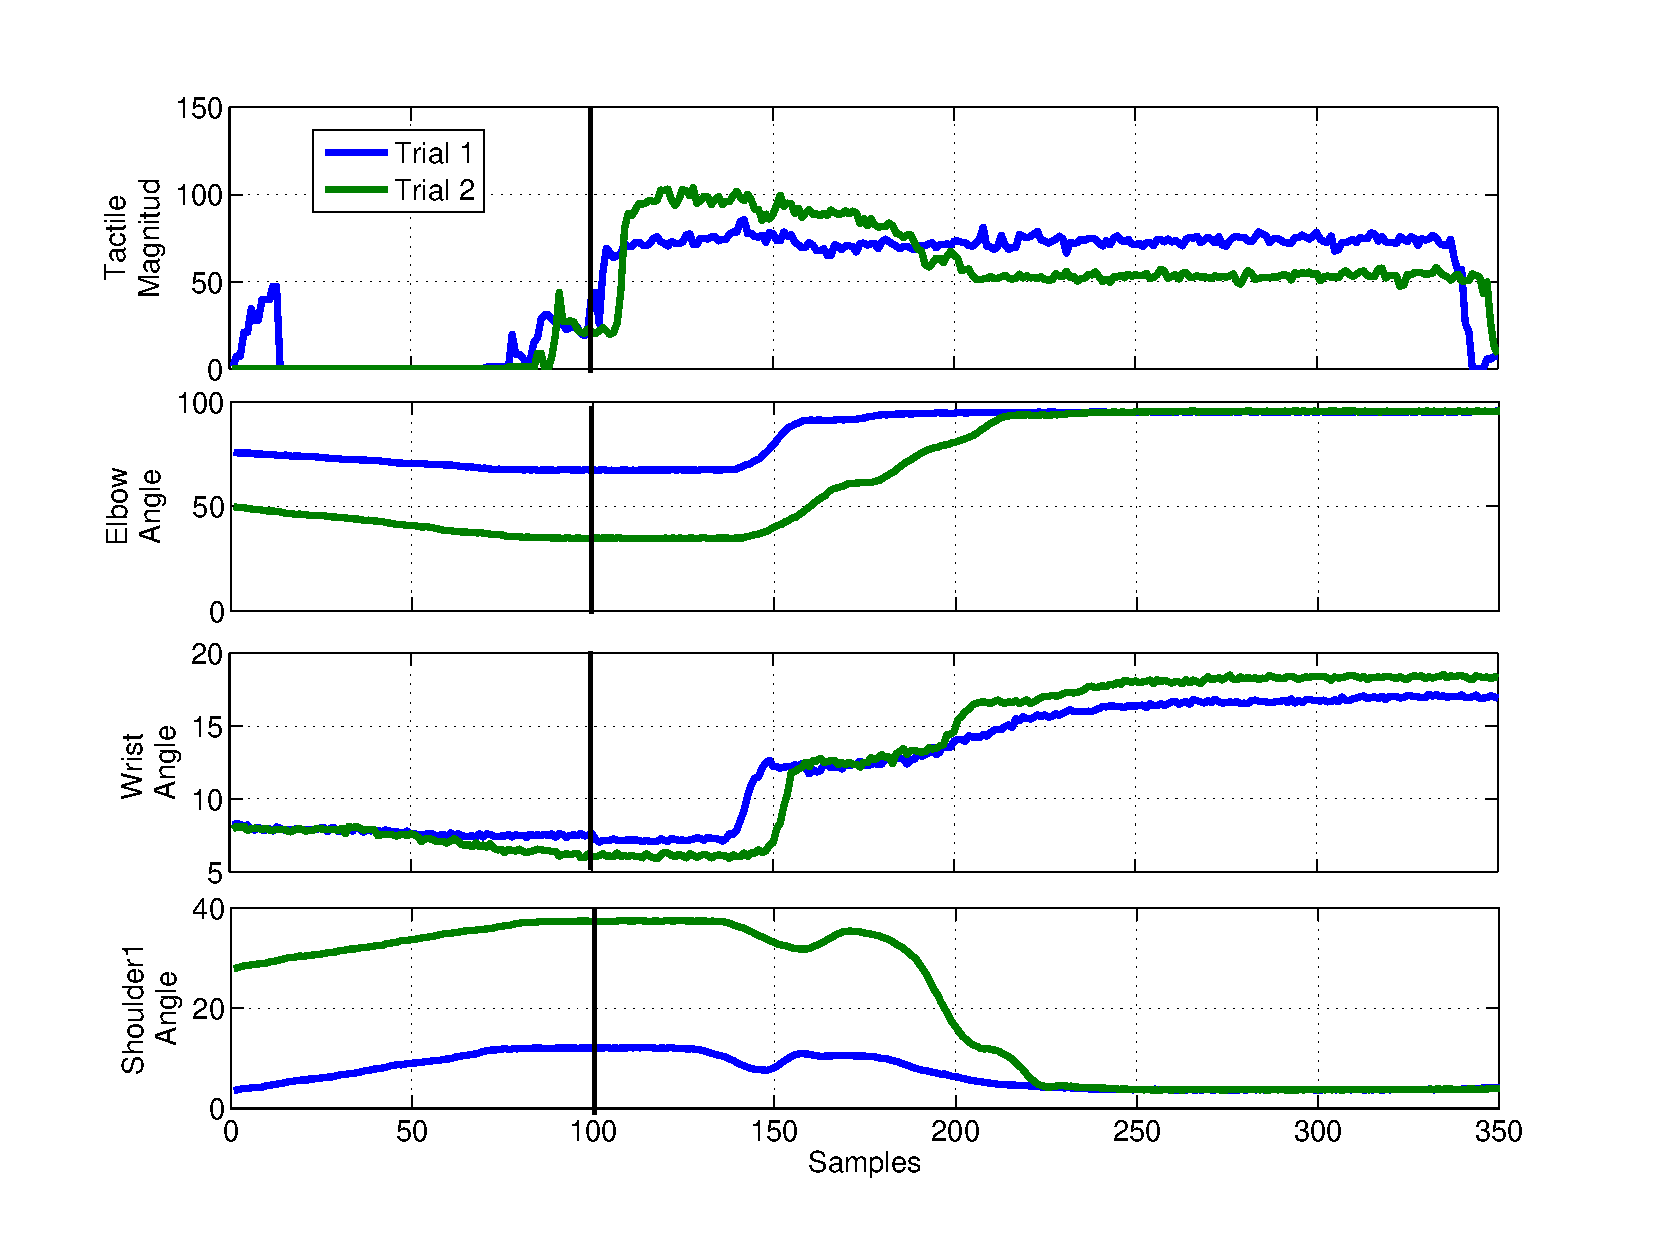
\includegraphics[width=3.5in]{./figures/GraspingData1.eps}
%% }\caption{The figure presents the trajectories followed by two
%% different grasping sequences of a same object. We can observe that
%% the tactile sensor response capture the variation in the different
%% trajectories. The magnitude of the tactile vector is the vectorial
%% summation of the forces present in each tactile sensor considering
%% the current geometry of the hand.} \label{fig:AnglesPlot}
%% \end{figure}

%% \begin{figure}[tbp]
%% \centerline{
%% 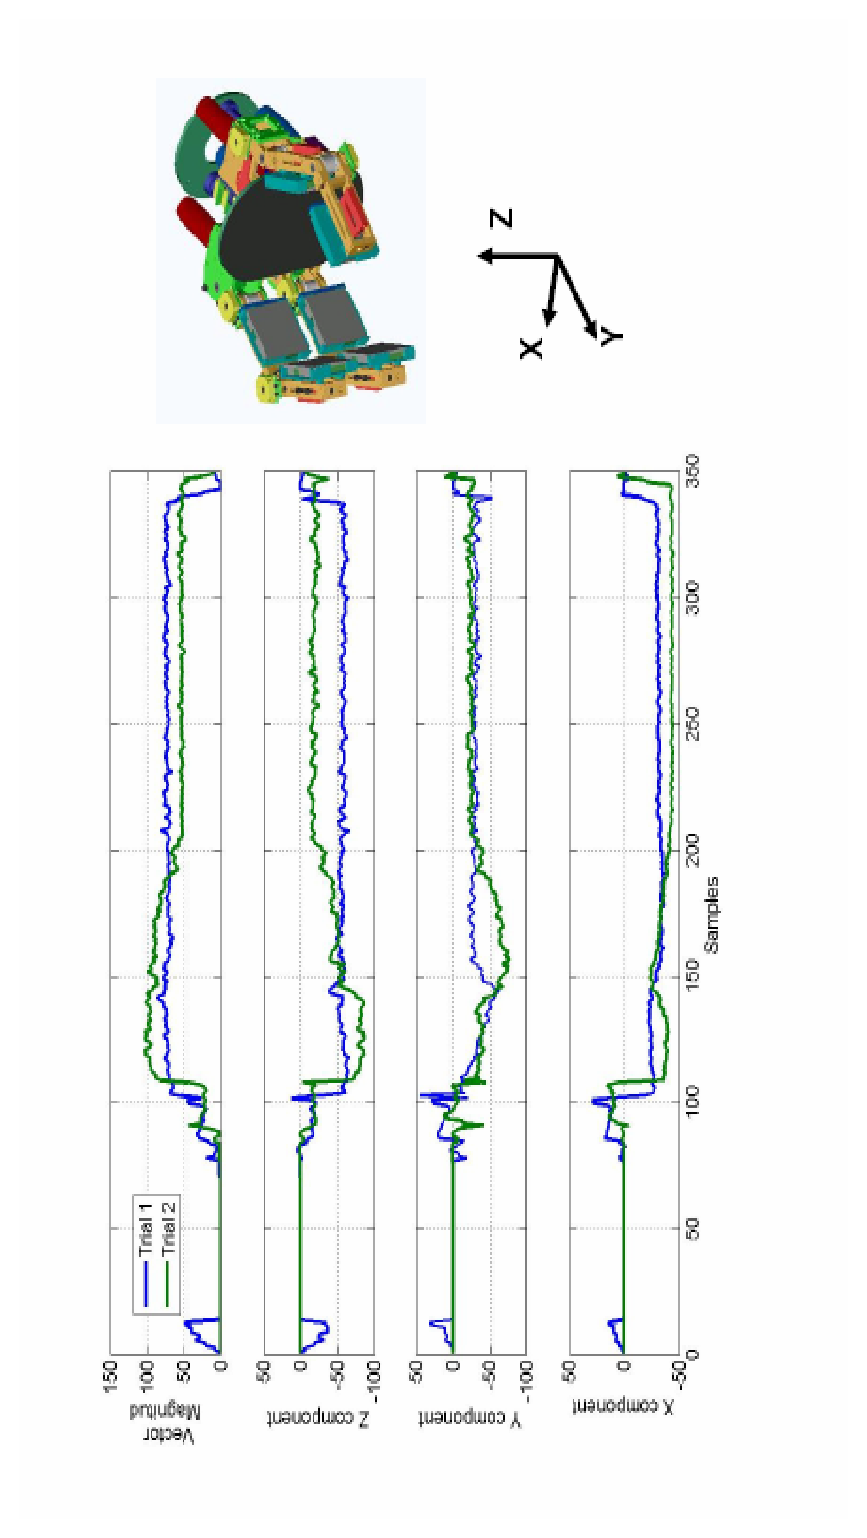
\includegraphics[height=3.2in, angle=270]{./figures/TactileComp.eps}
%% }\caption{The magnitude of the tactile vector is the vectorial
%% summation of the forces present in each tactile sensor considering
%% the current geometry of the hand.} \label{fig:TactileComp}
%% \end{figure}

The grasping described in Section~\ref{sec:controlling} was
evaluated by presenting different objects to the robot and by
counting the number of successful grasps. We chose objects of
different size and shape: a plastic bottle, a plastic rectangular
box, a porcelain cup and a plastic cup (see
figure~\ref{fig:Objects}). Some of the objects were partially
filled, so that the weight was roughly uniform among all objects
(about 220-250 grams, see Table~\ref{tab:objects}). The robot had
no prior knowledge about these objects.

Each object was presented to the robot more than 20 times and
randomly placed on the table. Overall the number of grasping
trials was 94, of which only 7 were not successful. In some of
these trials, the robot managed to grasp the object, but was not
able to hold it because the grip did not produce enough friction.
In a few cases the tactile sensors failed to detect the object and
the exploration was aborted before the object was actually grasped
(more details are reported in Table~\ref{tab:objects}).

As a further validation, we clustered the haptic information
originated from the grasping. We collected the hand feedback at
the moment the robot lifted the object; the idea is that given the
intrinsic compliance of the hand, its configuration and the force
exerted by each joint depend on the shape of the object being
grasped. The hand feedback was clustered by means of a Self
Organizing Map (SOM). The results show that the bottle, the
rectangular box and the cups form three clusters. Unfortunately
the clusters formed by the two cups are not clearly
distinguishable. This is probably due to the fact that the hand
grasped the objects from the top, and that in that part the two
objects are quite alike (both are circular with similar diameter).
In these cases the limited number of fingers (three) made it hard
to distinguish between the cylindrical and conic shape of the
cups. Together the results prove that the \emph{grasping} behavior
of the robot is reliable. The high number of successful trials
shows that the haptic feedback manages to drive the robot during
the exploration until it finds the object and grasps it. This is
further demonstrated by the clustering, which show that the
behavior allows extracting meaningful information about the
physical properties of the objects (i.e. their shape).


\section{Analysis of tactile data}


\subsection{Sensitivity Required}

But first we would like to emphasize the difference between
compliant sensors and state of the art tactile sensors by
presenting a couple of evaluations.

In figure~\ref{fig:TouchEgg}, we observe an example of the
compliant sensors working. In this case, the fingers of the hand
close until contact is detected. We see that the sensitivity of
the tactile sensors is enough to detect the contact with an egg
and avoid the fingers to exert excessive force to break it. It is
important to note that the sensors conform to the egg which helps
to constrain the egg's motion and distributes the force reducing
the pressure on the egg's surface.

In order to contrast our compliant sensor features, we refer to
the sensor developed by
Maheshwari~and~Saraf~\cite{touchsensorScience}. This sensor is
capable of recovering the shape embossed on a US penny, but it is
not capable of conforming to the egg. Moreover, given that it is
flat and rigid, the force applied concentrates in a small area
which causes great stress in that area. As reference, this sensor
needs at least $9KPa$ to detect contact. This stress can cause a
fracture on the egg surface.

We further evaluate the compliant sensors on a more delicate task.
In figure~\ref{fig:PaperGentle}, we observe the robot gently
gripping a paper cylinder while the cylinder is only slightly
deformed. There is a weight on the base to keep the cylinder in
place. The weight's size is smaller than the circle of the base so
it does not affect the cylinder structure. The robot's hand
approaches the cylinder by the side. Once the tactile sensors
detect the contact, the robot rotates its finger and closes the
thumb slowly up until contact is detected. The sensitivity of the
compliant tactile sensor is such that the cylinder is only
slightly deformed. On the other hand, we can observe in
figure~\ref{fig:PaperNoGentle} that the cylinder is deformed when
no tactile feedback is used.

The sensitivity of our compliant tactile sensor is in general high
because of its structural design. We can think of the overall
shape of the sensor as an hemisphere, therefore, when the sensor
first comes in contact with a locally flat surface only a point
-in theory- is touched. The stress in that point is high causing
the structure to deform making detection possible. This feature,
allows the sensor to work well with most surfaces.

In contrast, the flat rigid surface of the sensor previously
mentioned~\cite{touchsensorScience} distributes the force applied.
For example, if this sensor comes in contact with a flat surface
of the same size as the sensor's surface, a large force will be
needed to detect the contact. The experiment with the paper
cylinder has little likelihood to work with this sensor, because
the rigidity of its surface will deform the cylinder without
detection.

The sensitivity of the sensor is within the range of human
sensitivity. Human sensitivity is around 0.3~N to 1.0~N as
mentioned in ~\cite{touchsensorScience} and our tactile sensor's
minimum detectable normal force is around 0.1~N in the magnetic
version and 0.01~N in the optical.


Science Paper... Many tactile sensors have only been tested on the
bench. Focus on get density... However, no much attention to the
data produced. We for example believe that those properties are
important but not as much as the shape.
%


\begin{figure}[tbp]
\centerline{
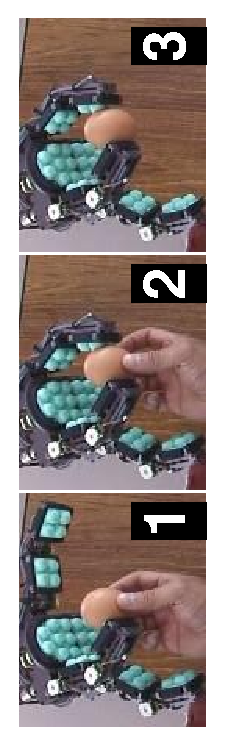
\includegraphics[height=\columnwidth, angle=270 ]{./figures/EggSeq.eps}
} \caption[Grabbing an egg]{In this sequence we observe the hand
closing on a egg. This task is easier than the one shown in
figure~\ref{fig:PaperGentle}. If we observe carefully 3. we can
notice the properties of the tactile sensors. They detect the
contact but also conform to the object increasing friction and
making an stable grasp possible.} \label{fig:TouchEgg}
\end{figure}

\begin{figure}[tbp]
\centerline{
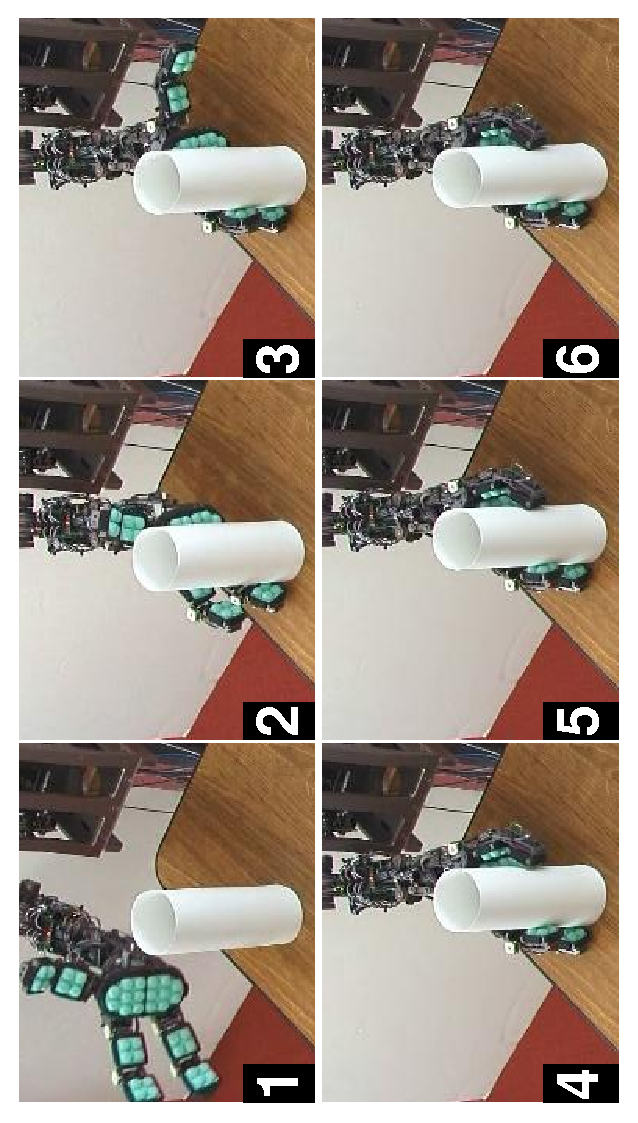
\includegraphics[height=\columnwidth, angle=270 ]{./figures/PaperGentle.eps}
} \caption[Gently grabbing a paper cylinder]{In this sequence we
observe the robot approaching a cylinder made of paper bond. This
cylinder has a weight in its bottom. The robot can detect the
first contact, oppose its thumb and move the thumb, gently
stopping when detecting the contact. The tactile sensors are
sensitive enough to detect the cylinder without crushing it.}
\label{fig:PaperGentle}
\end{figure}

\begin{figure}[tbp]
\centerline{
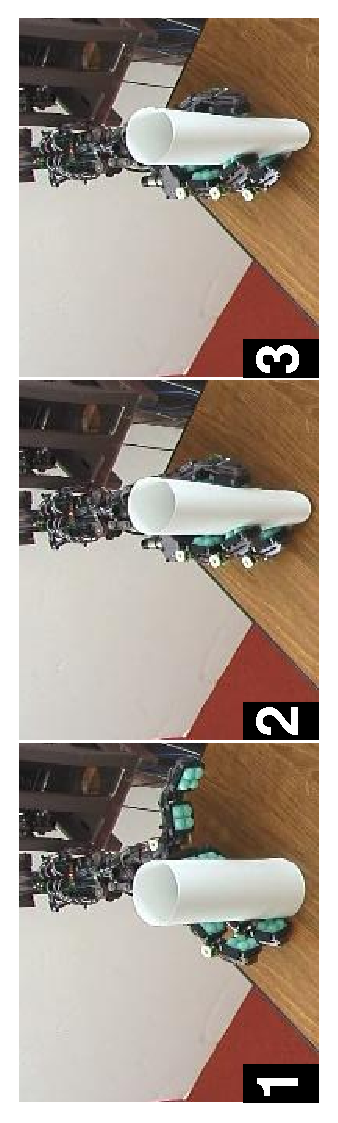
\includegraphics[height=\columnwidth, angle=270 ]{./figures/PaperNoGentle.eps}
} \caption[Crushing paper cylinder]{In this sequence the robot
closes its fingers without using tactile feedback. As a
consequence they crush the object.} \label{fig:PaperNoGentle}
\end{figure}





%\subsection{Slippage}
%\label{sec:slippage}
%
%In this section we present our implementation of slippage
%detection using the compliant sensors. Although controlling
%slippage can be useful in several manipulation tasks, we focus on
%avoiding slippage when lifting.
%
%
%Sensing slippage is not an straight-forward task since the
%phenomena is not quite understood. If we observe humans, our skin
%has innervations that respond to fast motions on the surface.
%These innervations are the Meissner's corpuscles. They are
%specialized on detecting vibrations. Those vibrations are, in
%principle, related to the catch and release effect caused by an
%object sliding on the surface of the skin. This has inspired other
%researchers to build tactile sensors with the capability of
%detecting vibrations using accelerometers\cite{howe89sensing}.
%
%In our case we do not rely on this principle. Instead, we measure
%the change of the force applied on the direction of the lifting.
%
%We illustrate this principle on the following experiment. We use
%the the cylindrical bottle ($mass=0.179 Kg$, $diameter=92 mm$,
%$height=216 mm$) shown in figure~\ref{fig:slipseq}. The robot
%approaches the bottle by the side, touches it and subsequently
%rotates the thumb to grab the object. Since it is the first time
%it works with the bottle, it closes its thumb and index finger
%gently until contact with the object is detected. At this point,
%it closes the fingers more to deflect the sensors. This is
%necessary in order to obtain reliable readings from forces applied
%in directions parallel to the base of the sensors. In
%figure~\ref{fig:tactileref} we can observe the direction of the
%forces on the tactile sensors. In this experiment, we use only the
%tactile sensors on the distal phalanges of the fingers. The force
%normal to the tactile sensor surface is in the X direction, and
%the ones parallel are in the plane Y-Z.
%
%When the fingers are closed on the object, the forces in X
%increase. The forces in Z (on the direction of gravity) and the
%forces in Y also change due to the deformation of the sensors.
%This deformation depends, at this point, on the angle of incident
%between the tactile sensor and the surface of the object and not
%on the weight.
%
%When the robot starts moving its hand upwards, that is indicated
%by the increment of elbow angle figure~\ref{fig:slip}, the force
%in Z increases in magnitude because the weight of the object pulls
%the sensors down. Assuming that the motion is linearly upwards and
%that the object does not rotate, the force should remain somewhat
%stable. The exception is at the beginning of the lifting where the
%dynamics of the motion are noticeable. The event just described is
%illustrated on the right side of figure~\ref{fig:slip}.
%
%On the left side of figure~\ref{fig:slip}, we see that the
%behavior is different. The total force goes back to zero while the
%fingers are still closed. This is because the object slipped from
%the hand. A sequence of images of the slippage is shown in
%figure~\ref{fig:slipseq}. It is important to notice in this figure
%that the bottle moves downwards but also towards the front. That
%is, the bottle rotates on the finger tips of the hand.
%
%If we now return to figure~\ref{fig:slip}, we can see the dynamics
%of the sensors/object interaction. After the point B, in the
%figure, the total force becomes negative because the friction with
%the object pulls the sensors down. This event is indicated by an
%increment on the elbow angle. While the total force is negative,
%there is a slight positive slope on the force that indicates some
%slippage. But more importantly, the angle between forces Z and Y
%in the thumb changes smoothly showing the rotational slippage.
%Subsequently, the object stops pulling down the tactile sensors
%when it touches the table. At point C in figure~\ref{fig:slip},
%the fingers are opened.
%
%
%In order to detect slippage, we observe the total tactile force
%while the fingers are closed and the arm moves upwards. If we
%detect a positive slope, we conclude that there is slippage. We
%can observe this in figure~\ref{fig:slip}. From point B to C there
%is a large positive slope. The slope is presented on the top plot
%for reference. From points E to F, there is a slight slip that
%stops and the grasp stabilizes.
%
%The response time of this slip detector is not as fast as it woudl
%be required to adjust the force instantly. Instead, a new attempt
%to lift the object is done if slippage has been detected. The
%current limitation of these sensors is that computation is done
%off-board. However, the hardware on the sensors have the
%capability of doing this calculation faster.
%
%
%\begin{figure}[htbp]
%\centerline{
%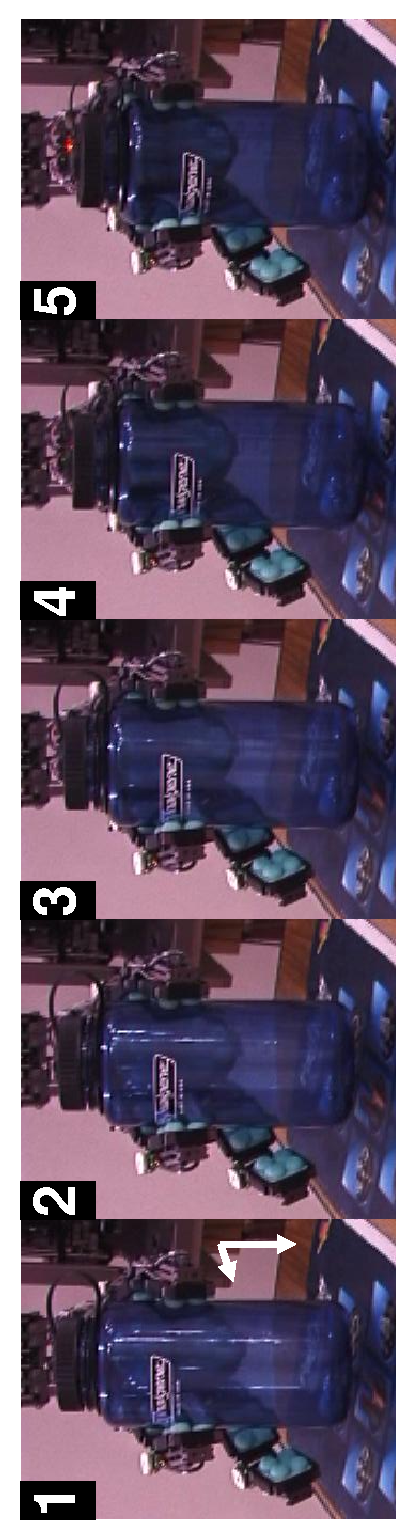
\includegraphics[height=\columnwidth, angle=270 ]{./figures/Slippage.eps}
%} \caption[Bottle slipping]{From 1 to 5 we observe the bottle
%slipping. The bottle moves downwards and towards the front. The
%motion towards the front is not linear but circular.}
%\label{fig:slipseq}
%\end{figure}
%
%
%
%
%
%
%
%It is important to remember that the data comes from a controlled
%experiment where the lifting is done only with the thumb and the
%index finger. Neither the palm nor the middle finger are used. In
%general, this robot is designed to do whole body grasping as
%opposed to precision grasping. In some cases, an object will come
%in contact with the fingers on spots where the fingers are not
%fully covered with the skin. In that case the slippage detection
%is not possible.
%
%\begin{figure*}[htbp]
%\centerline{
%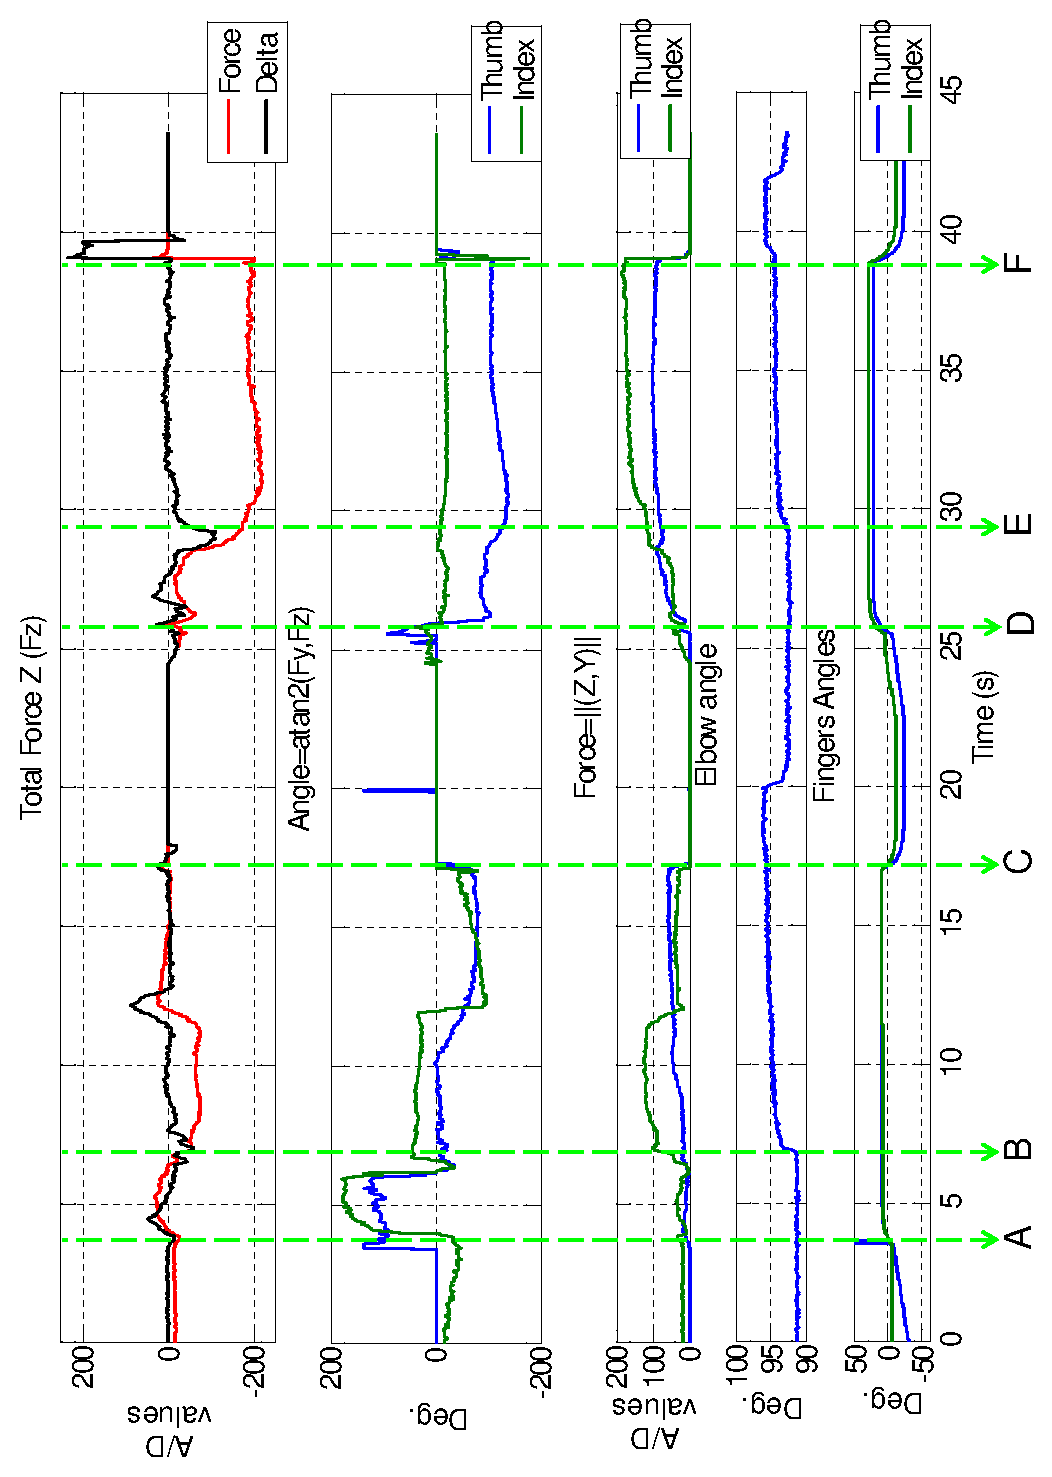
\includegraphics[height=\textwidth, angle=270 ]{./figures/ThesisSlipX.eps}
%} \caption[Tactile forces when lifting an object]{Tactile forces
%in two different lifting events. For details see
%section~\ref{sec:slippage} } \label{fig:slip}
%\end{figure*}
%


%Pushing the bottle upwards twice. Sample time 100 ms. Compute
%delta. Filtered in 8 tap average filter. The second plot is
%integration. Done this way so it is independent of the force
%required.




\section{Limitations of the implementation}
\label{sec:imp:limitations}


 The current implementation works well
with objects whose height is greater than 0.120 m. This limitation
can be removed by rotating the hand so that the index and middle
finger end up positioned in top of the object. This movement also
covers the case when an object is knocked over during the
interaction. However, no all the objects can be handled with the
current size of the hand.

The size of the fingers is a current limitation imposed by the
original design which used larger tactile sensors. The size of the
fingers and the coupling of their phalanges limits the size of the
objects that can be manipulated. This limitation can be removed by
building a smaller version. The current configuration of the hand
is not adequate for all the cases. For instance, it would be
useful to be capable of reorienting the palm.

The implementation also fails when the object comes in contact
with the hand or arm in regions where there are not tactile
sensors. This occurs even when the objects are large.

The spatial resolution of the tactile sensors also limits current
implementation because some features of the objects are not
differentiable. That is the case of the handle of a coffee cup.
This could be solved with smaller version of the tactile sensors.



\section{Summary}
\label{sec:conclusions}

We have described the design of a behavior that allows a humanoid
robot to grasp objects without prior knowledge about their shape
and location. We summarize here our approach and the lessons we
learned:
%
\begin{itemize}
%
\item Give up precision, explore instead. Sometimes in robotics we
struggle to have robots as precise as possible in performing the
tasks for which we program them. We found that exploration can be
more effective in dealing with uncertainties.
%
\item Be soft. Exploration must be gentle if we want to avoid
catastrophic effects on either the robot or the
objects/environment. The mechanical design of the robot proved
helpful in this respect.
%
\item Sense and exploit the environment. If inquired, the world
can provide useful feedback; however the robot must be able to ask
the right questions (interact) and interpret the answers (have
appropriate sensors).
%
\end{itemize}

We endowed the robot with the minimum capabilities required to
explore the environment. These include a simple ability to detect
visual motion, a way to control the arm to roughly reach for
objects and a set of explorative primitives. Haptic feedback
drives the exploration and allows the robot to successfully grasp
objects on a table.

We further analyzed the tactile data obtained from the interaction
with the objects and implement methods to detect slippage and
external forces acting on an object being held. We also showed
that the information generated can be potentially used to learn
physical properties of objects like shape. This was possible in
part because of the properties of the tactile sensors, whose
advantages were further evaluated in this chapter.


In sensitive manipulation, we are interested in studying methods
to improve the perceptual abilities of robots by exploiting the
physical interaction with the environment. In this thesis, we have
shown how haptic feedback can significantly improve this
interaction thereby enhancing the robot's ability to learn about
the environment.

Finally, it is worth saying that, to better illustrate our point,
we deliberately took a somewhat extreme approach with respect to
relying primarily upon tactile sensory information. We certainly
believe that future robots will have to take advantage of the
integration of all sensory modalities.


\newpage


\section{Extra information}




\label{sec:imp:timing}

In table~\ref{tab:feedback}, we observe that the feedback
information is available at different frequencies. The low level
motor control receives the information from the encoders and
potentiometers at 500Hz. This frequency is adequate for force
control in the series elastic actuator and for the position
control of the limbs.

The tactile feedback is sent to a daemon in a linux node. The
information is updated at about 55 Hz. However, the tactile
sensors can detect events at higher frequencies using its local
microcontroller. Force and/or position feedback from the hand arm
and head are sent to the linux nodes from their respective low
level controllers. However, they are only available at 12.5 Hz to
the linux nodes because of communication delays.

This information shows that the behaviors implemented are
constrained in speed by the feedback frequency. Therefore, the
control architecture works at different speeds that is slow at the
higher levels controllers and faster at the low levels. This
structure is considered analog to the control loops in humans. A
consequence of this structure is that the right sensing has to be
used for a given task. For example, if we want to detect and avoid
slippage, the sensing and the reaction have to be executed at the
right level to work.


\begin{table}[htb]
  \caption[Feedback sampling frequency]{Feedback sampling frequency}
  %
  \label{tab:feedback}
  %
  \centering
  \begin{tabular}{|l|r|r|}
    \hline
    Name& Period (s)&Frequency (Hz)\\
     %       & (s)&(Hz) \\
    %&Object& W(Kg)&Trials&Fail&Contains \\
    \hline
    Low level motor control&0.002&500.00\\
    High level tactile feedback & 0.018 & 55.55\\
    High level position feedback &0.080 & 12.50\\
    High level force feedback &0.080 & 12.50\\

    \hline
  \end{tabular}
\end{table}


\subsection{Old Implementation}


We describe the implementation of a behavior that allows the robot
to grasp objects.

We will refer to figure~\ref{fig:expbehaviors} to explain the
interaction between behaviors. It should be noted in the figure
that a behavior can be inhibited or enabled. When a behavior is
inhibited, it will not send commands. When a behavior is enabled,
the behavior can be either active or inactive. When, it is active,
it is sending commands because the programmed conditions have been
meet.

In figure~\ref{fig:expbehaviors}.1, the robot's arm is in a safe
position. A safe position above the table is defined for this
implementation. We start by describing the \emph{reaching
behavior}. The attention system, previously described, detects
when a experimenter waves an object in front of the robot. The
head tracks the object until it remains stationary within the
workspace of the arm. If the arm is in a safe position, the robot
moves the arm towards the object
(figure~\ref{fig:expbehaviors}.2). Reaching is not accurate enough
to guarantee a correct grasp. Since no three dimensional
information is available the arm reaches a region above the object
(see Section~\ref{sec:reaching}). At this point the \emph{reaching
behavior} enables the other behaviors
(figure~\ref{fig:expbehaviors}.3). The robot computes the
directions $v_1$, $v_2$, and $v_3$ and explores using the
following three behaviors: \emph{depth behavior}, moves the hand
``downwards'' vertically $v_3$; \emph{hovering behavior}, moves
the hand back and forth along $v_1$;\emph{pushing behavior}, moves
the hand along $v_2$;


The \emph{depth behavior} moves the hand along the direction of
the optical axis of the camera and adjusts the height of the hand
with respect to the object/table. To avoid crashing the hand into
the table this behavior is inhibited when the infrared proximity
sensor detects an obstacle (usually this happens close to the
table). The \emph{hovering behavior} and the \emph{depth behavior}
are activated at the beginning of the exploration. The goal of
this initial phase is to adjust the position of the hand until the
index finger touches the object. This allows adjusting the
position of the hand along the directions $v_1$ and $v_3$. During
the exploration the arm stops when the hand detects the object, to
avoid pushing it away or knocking it over; if no contact is
detected, the amplitude of the exploration is extended (this
increases the probability to touch the object in case the reaching
error is large). The exploration terminates when the contact with
the object is detected by any of the tactile sensors placed on the
index finger. At this point the \emph{hovering behavior} is
suspended and the \emph{pushing behavior} activated
(figure~\ref{fig:expbehaviors}.4). The ``pushing'' movement along
$v_2$ brings the palm in contact with the object while the
\emph{depth behavior} takes care of maintaining the correct
distance with the table. When the robot detects contact on the
palm the exploration stops and the \emph{grasping behavior} is
activated. The \emph{grasping behavior} simply closes the fingers
to a specific position. The low impedance of the joints allows the
fingers to adapt to the different objects being grasped.

[Include here the grasping and the lifting] with feedback.

Figure~\ref{fig:sequence} reports an example of the robot grasping
a porcelain cup. The relation between the behaviors and the
actions of the robot are presented in figure~\ref{fig:bsteps}. The
\emph{grasping} behavior proved to be quite reliable, as several
repeated tests show in Section~ \ref{sec:results}

\subsection{Interaction}

We now turn our attention to the data produced by the compliant
tactile sensors when interacting with an object. We can observe a
sample of this in figure~\ref{fig:AnglesPlot}. In this figure we
observe the trajectory followed by the arm in two different
grasping sequences. The trajectory is represented by the angles of
the elbow, wrist, and shoulder. The angle of the shoulder shown is
the one that moves the arm up.

These differences between the trajectories are reflected in the
tactile sensors' readings as shown in the top plot of
figure~\ref{fig:AnglesPlot}. In this plot, the magnitude of the
tactile vector is the vectorial summation of the forces exerted in
each tactile sensor considering the current geometry of the hand.

We can see that the magnitude increases when the fingers are
closed around the object. In the first trial, the magnitude
remains quite constant while in the second there is a greater
change due to the different trajectory of the elbow and the
shoulder.

\begin{figure}[tbp]
\centerline{
%\includegraphics[width=2.0in, angle=270 ]{./figures/tactref.eps}
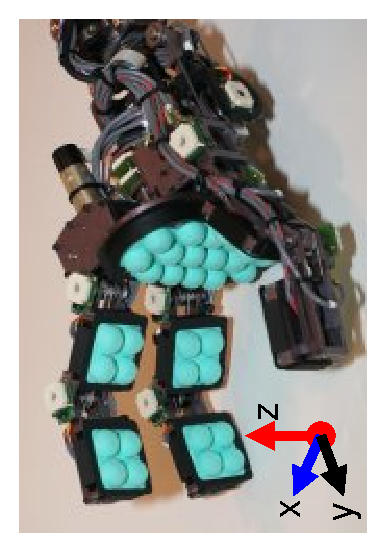
\includegraphics[width=2.0in, angle=270 ]{./figures/refaxis.eps}
} \caption[Axis of reference for tactile sensors]{Axis used to
reference the forces acting on the tactile sensors on the hand.}
\label{fig:tactileref}
\end{figure}



A more detailed plot of the response of the tactile sensors is
presented in figure~\ref{fig:TactileComp}. In this figure we can
observe that the Z and the Y components change as the arm follows
a trajectory. The Z component of the second trial (in green)is
smaller than the first because the object is in contact with the
hand in regions with no tactile sensors. Finally, the X component
does not go to zero mainly because the compliant sensors are not
calibrated. However, we do not rely on this condition to evaluate
the grasp.



Further analysis of this information allows us to detect events
such as slippage or contact of the object with an external
element.

%\section{The second part}
%
%
%\section{Kinematics}
%
%\begin{figure}[tbp]
%\centerline{
%\includegraphics[width=4.0in, angle=0 ]{./figures/kinebrazo.eps}
%} \caption{Kinematics of the arm. The axis are numbered from 0 to
%5 going from the shoulder to the wrist. The initial reference is
%on the center of the neck of the robot.} \label{fig:kinebrazo}
%\end{figure}
%
%
%\section{REUSE}




%%
%\subsection{The hand and the tactile sensors}
%%
%The hand consists of a palm, a thumb, a middle and an index finger
%(figure~\ref{fig:TactileSensors}). Each one of the fingers has two
%phalanges that can be opened and closed. The thumb and the middle
%finger can also rotate. These rotations allow the thumb to oppose
%to either the index or the middle finger. The total number of
%degrees of freedom in the hand is 8. All joints in the hand are
%equipped with an optimized version of the Series Elastic Actuators
%\cite{actuator}; the fingers have low mechanical compliance to
%soften the contact with the objects during grasping.
%%mechanical compliance of the fingers is very low to %which
%%provide force feedback and reduce the mechanical impedance of the
%%fingers.
%The hand is underactuated and driven by only 5 motors: three
%motors open and close each finger, whereas two motors control the
%rotation of the thumb and middle finger. The phalanges of each
%finger are mechanically coupled. However, due to the presence of a
%Series Elastic Actuator in the joint, independent motion is
%achieved when the proximal phalange blocks (for example, as a
%result of contact with an object). This elastic coupling allows
%the hand to automatically adapt to the object it grasps. Finally,
%position feedback is obtained through potentiometers mounted in
%all joints and encoders in the motors.
%%
%%
%\begin{figure}[tbp]
%\centerline{
%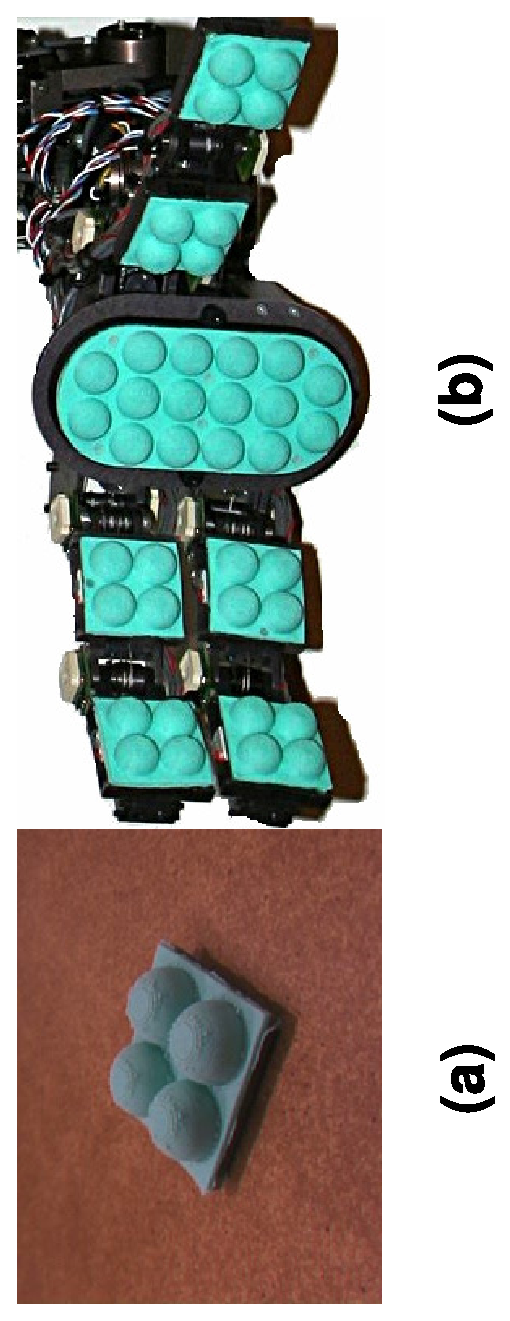
\includegraphics[width=1.0in, angle=270 ]{./figures/Tactiles.eps}
%} \caption{OBRERO's hand and detail of the tactile sensors. (a)
%Group of four tactile sensors. The deformation of each of them is
%measured by a total of four sensors. (b) Tactile sensors mounted
%on the hand.} \label{fig:TactileSensors}
%\end{figure}
%%
%The tactile sensors mounted on the hand were designed to satisfy
%the needs of robotic tasks. Each unit has a dome-like sensor (see
%figure~\ref{fig:TactileSensors}a) made of silicon rubber. At the
%tip of the dome we embedded a small magnet, whose position is
%measured by four hall-effect sensors placed at the dome's base. By
%sensing the position of the magnet the deformation of the dome is
%estimated. The sensors are very sensitive and capable of detecting
%a minimum normal force of 0.098N. The shape of the sensors favors
%contact with the environment from any direction, as opposed to
%most of the tactile sensors which are flat. The high deformability
%and the properties of the silicon rubber allow the sensors to
%conform to the objects, thus increasing friction and improving
%contact detection. In this particular implementation, we used the
%``magnetic'' version of these tactile sensors, however, an optical
%version has also been tested. The description of the design and
%the analysis of these sensors can be found in \cite{etorresjSoft}.
%
%Groups of tactile sensors were placed on the hand. Two groups of
%four were placed on each finger (a group in each of the two
%phalanges) and 16 on the palm. A detail of the palm and fingers
%can be observed in figure~\ref{fig:TactileSensors}b. Each one of
%these tactile units uses four sensors to determine the contact
%forces. This means that overall the tactile feedback consists of
%160 signals. At the base of the palm, where for practical reasons,
%we were not able to mount these tactile sensors, we placed a
%smaller infrared proximity sensor. To summarize, the hand has 5
%motors, 8 DOF, 8 force sensors, 10 position sensors, 160 tactile
%sensors and an infrared proximity sensor.
%

%======REUSE
%
%Motivated by these ideas,  we have favored the sensing
%capabilities over the precision in the design of OBRERO's limb.
%The limb has force control, low mechanical impedance as well as
%position and force sensing.
%
%
%While tactile information will dominate, \textit{sensitive
%manipulation} also can benefit from visual and auditory
%perception.  Such information will be used by the robot to improve
%the efficiency of manipulation, rather than be an essential
%prerequisite. Vision can give a quick estimate of an object's
%boundary or find interesting inhomogeneities to probe.  Sound is
%also a very important clue used by humans to estimate the position
%of an object and to identify it. We have conducted experiments to
%take advantage of this fact in \cite{tapping}.  The robot OBRERO
%has a 2 degree-of-freedom head that includes vision and sound. The
%camera has two optical degrees of freedom; focus and zoom. Focus
%is very useful to obtain depth information and zoom helps to
%obtain fine details of an image. The vision system will try to
%take advantage of natural cues present in the environment such as
%shadows \cite{fitzpatrick04power}.
%
\section{Introduction}
%
Recent work in developmental robotics has emphasized the role of
action for perception and learning
\cite{metta03early,natale04learning,natale05from}. Developmental
psychology, on the other hand, recognizes that motor activity is
of paramount importance for the correct emergence of cognition and
intelligent behavior
\cite{gibson88explore,streri93Seeing,bushnell93motor,hofsten04motor}.
All embodied agents, either artificial or natural, have numerous
ways to exploit the physical interaction with the environment to
their advantage.

In robotics, actions like pushing, prodding, and tapping have been
used for visual and auditory perception respectively
\cite{metta03early,etorresjara05tapping}. More articulated
explorative actions or grasping might increase these benefits, as
they give direct access to physical properties of objects like
shape, volume and weight.
%
Unfortunately, all these aspects have not been extensively
investigated yet. One of the reasons for this is that controlling
the interaction between the robot and the environment is a
difficult problem \cite{volpe90real}, especially in the absence of
accurate models of either the robot or the environment (as it is
often the case in non-engineered environments).
%
The design of the robot can ease these problems. We know for
example that having a certain degree of elasticity in the limbs
helps to ``smooth''  and control the forces that originate upon
contact. Another approach is to enhance the perceptual abilities
of the robot. Traditional robotic systems in fact have perceptual
systems that do not seem adequate for grasping. Haptic feedback in
particular is often quite limited or completely absent. This is
because, unfortunately, most of the tactile sensors commercially
available are inadequate for robotics tasks: they are only
sensitive to forces coming from a specific angle of incidence,
rigid and almost frictionless.

OBRERO \cite{obrero}, described in paper, was designed to overcome
these limitations. It is equipped with series elastic actuators,
which provide intrinsic elasticity and force feedback at each
joint. The hand is equipped with tactile sensors
(Section~\ref{chap:TactileSensors}) which provide a deformable and
sensitive interface between the fingers and the objects.

In this paper, we report a series of experiments where OBRERO
exploits its sensing capabilities to grasp a number of objects
individually placed on a table. No prior information about the
objects is available to the robot. The use of visual feedback was
voluntarily limited. Vision is used at the beginning of the task
to direct the attention of the robot and to give a rough
estimation of the position of the object. Next, the robot moves
its limb towards the object and explores with the hand the area
around it. During exploration, the robot exploits tactile feedback
to find the actual position of the object and grasp it. The
mechanical compliance of the robot and the control facilitate the
exploration by allowing a smooth and safe interaction with the
object. Results show that the haptic information acquired by the
robot during grasping carries information about the shape of the
objects. Further analysis of the tactile data allows us to detect
slippage and sense forces applied over the object being held by
the robot.

\section{Haptic feedback, perception and action}
\label{sec:background}

In adults, several studies have revealed the importance of
somatosensory input. For example Johansson and Westling
\cite{Johansson90Tactile} have studied in detail what feedback is
provided by the skin during object lifting tasks and how it is
used to control the movements of the fingers. The results of these
experiments proved the importance of somatosensory feedback: they
showed that human subjects had difficulties avoiding object
slipping when they had their fingertips anesthetized, even with
full vision \cite{johansson91how}.

Haptic feedback has an important role for object perception as
well. Lederman and Klatzky \cite{lederman87hand} identified and
described a set of motor strategies named \emph{exploratory
procedures} used by humans to determine properties of objects such
as shape, texture, weight or volume.

Little is known concerning how infants use tactile sensing for
manipulation \cite{streri93Seeing}.
%Tactile sensing in neonates is very poorly known
%in contrast to the visual mechanism\cite{streri93Seeing}.
%However, tactile sensing provides information to children since
%his time in the wound.
In some circumstances children exploit tactile feedback to learn
about objects \cite{streri86Habituation}. Streri and P\^{e}cheux
measured the habituation time of newborns (2 months and 5 months
old) during tactile exploration of objects placed in their hands.
In this experiment children spent more time exploring novel rather
than familiar objects, even when they did not make visual contact
with the hand. %This experiment was repeated with visual feedback
%showing the same behavior.

Motor abilities of children are quite limited during the first
months of development. This does not prevent infants from using
their hand to engage interaction with the world. The importance of
motor activity for perceptual development has been emphasized in
developmental psychology \cite{hofsten04motor,gibson88explore}.
Researchers agree on the fact that motor development determines
the timing of perceptual development. In other words the ability
of infants to explore the environment would determine their
capacity to perceive certain properties. Accordingly, perception
of object features like temperature, size and hardness is likely
to occur relatively early in development, whereas properties
requiring more dexterous actions like texture or three dimensional
shape would emerge only later on (see \cite{bushnell93motor} for a
review).

\section*{Acknowledgement}
% optional entry into table of contents (if used)
%\addcontentsline{toc}{section}{Acknowledgment}
The work presented in this paper
has been supported by the \textsc{RobotCub} project (IST-2004-004370), funded by the
European Commission through the Unit E5 ``Cognitive Systems''. Moreover, it has
been partially supported by \textsc{Neurobotics}, a European FP6 
project (IST-2003-511492) and \textsc{Contact} (NEST 5010).




%

% references section
%%% this must be IEEEtran
\bibliographystyle{IEEEtran}
\end{document}

\bibliography{main}
